% This is "sig-alternate.tex" V2.0 May 2012
% This file should be compiled with V2.5 of "sig-alternate.cls" May 2012
%
% This example file demonstrates the use of the 'sig-alternate.cls'
% V2.5 LaTeX2e document class file. It is for those submitting
% articles to ACM Conference Proceedings WHO DO NOT WISH TO
% STRICTLY ADHERE TO THE SIGS (PUBS-BOARD-ENDORSED) STYLE.
% The 'sig-alternate.cls' file will produce a similar-looking,
% albeit, 'tighter' paper resulting in, invariably, fewer pages.
%
% ----------------------------------------------------------------------------------------------------------------
% This .tex file (and associated .cls V2.5) produces:
%       1) The Permission Statement
%       2) The Conference (location) Info information
%       3) The Copyright Line with ACM data
%       4) NO page numbers
%
% as against the acm_proc_article-sp.cls file which
% DOES NOT produce 1) thru' 3) above.
%
% Using 'sig-alternate.cls' you have control, however, from within
% the source .tex file, over both the CopyrightYear
% (defaulted to 200X) and the ACM Copyright Data
% (defaulted to X-XXXXX-XX-X/XX/XX).
% e.g.
% \CopyrightYear{2007} will cause 2007 to appear in the copyright line.
% \crdata{0-12345-67-8/90/12} will cause 0-12345-67-8/90/12 to appear in the copyright line.
%
% ---------------------------------------------------------------------------------------------------------------
% This .tex source is an example which *does* use
% the .bib file (from which the .bbl file % is produced).
% REMEMBER HOWEVER: After having produced the .bbl file,
% and prior to final submission, you *NEED* to 'insert'
% your .bbl file into your source .tex file so as to provide
% ONE 'self-contained' source file.
%
% ================= IF YOU HAVE QUESTIONS =======================
% Questions regarding the SIGS styles, SIGS policies and
% procedures, Conferences etc. should be sent to
% Adrienne Griscti (griscti@acm.org)
%
% Technical questions _only_ to
% Gerald Murray (murray@hq.acm.org)
% ===============================================================
%
% For tracking purposes - this is V2.0 - May 2012

\documentclass{acm_proc_article-sp}

\usepackage{graphicx}
\usepackage{caption}
\usepackage{subcaption}
\usepackage{url}
\usepackage{subfigure}
\usepackage{textcomp}
\usepackage{tikz}
\usetikzlibrary{arrows,positioning} 

% Redefines \@ptsize to make setspace happy
% \makeatletter
% \renewcommand{\@ptsize}{0}
% \makeatother

%Double-spaces the entire document
% \usepackage{setspace}
% \doublespacing

\begin{document}
%
% --- Author Metadata here ---
\conferenceinfo{ICMI}{'13 Sydney Australia}
%\CopyrightYear{2007} % Allows default copyright year (20XX) to be over-ridden - IF NEED BE.
%\crdata{0-12345-67-8/90/01}  % Allows default copyright data (0-89791-88-6/97/05) to be over-ridden - IF NEED BE.
% --- End of Author Metadata ---

\title{ChAirGest 2013 - Continuous Gesture Spotting and Recognition}
%
% You need the command \numberofauthors to handle the 'placement
% and alignment' of the authors beneath the title.
%
% For aesthetic reasons, we recommend 'three authors at a time'
% i.e. three 'name/affiliation blocks' be placed beneath the title.
%
% NOTE: You are NOT restricted in how many 'rows' of
% "name/affiliations" may appear. We just ask that you restrict
% the number of 'columns' to three.
%
% Because of the available 'opening page real-estate'
% we ask you to refrain from putting more than six authors
% (two rows with three columns) beneath the article title.
% More than six makes the first-page appear very cluttered indeed.
%
% Use the \alignauthor commands to handle the names
% and affiliations for an 'aesthetic maximum' of six authors.
% Add names, affiliations, addresses for
% the seventh etc. author(s) as the argument for the
% \additionalauthors command.
% These 'additional authors' will be output/set for you
% without further effort on your part as the last section in
% the body of your article BEFORE References or any Appendices.

\numberofauthors{2} %  in this sample file, there are a *total*
% of EIGHT authors. SIX appear on the 'first-page' (for formatting
% reasons) and the remaining two appear in the \additionalauthors section.
%
\author{
% You can go ahead and credit any number of authors here,
% e.g. one 'row of three' or two rows (consisting of one row of three
% and a second row of one, two or three).
%
% The command \alignauthor (no curly braces needed) should
% precede each author name, affiliation/snail-mail address and
% e-mail address. Additionally, tag each line of
% affiliation/address with \affaddr, and tag the
% e-mail address with \email.
%
% 1st. author
\alignauthor
Ying Yin\\
       \affaddr{Massachusetts Institute of Technology}\\
       \affaddr{}\\
       \affaddr{}\\
       \email{yingyin@csail.mit.edu}
% 2nd. author
\alignauthor
Randall Davis \\
       \affaddr{Massachusetts Institute of Technology}\\
       \affaddr{}\\
       \affaddr{}\\
       \email{davis@csail.mit.edu}
}

\maketitle
\begin{abstract}
We developed a gesture salience based hand tracking method and a gesture spotting method based on
concatenated hidden Markov models.
A 3-fold cross validation using the ChAirGest development data set gives an F1 score of 0.900
and an accurate temporal segmentation rate (ATSR) of 0.923. The average final score is 0.901.
\end{abstract}

%A category including the fourth, optional field follows...
\category{H.5.2}{Information Systems}{Information Interfaces and
Presentation}[User Interfaces]

\keywords{Gesture recognition, HMM, gesture spotting}

\section{Introduction}
The goal of ChAirGest 2013 challenge~\cite{Ruffieux2013} is to spot and recognize gestures independent of
users. We present our approach, highlighting two main contributions: 
improved hand position detection and gesture spotting.

Our work builds on several related works. Marcos-Ramiro et al.~\cite{marcos2013} developed a method of computing hand likelihood maps based on RGB videos. 
Our hand tracking method is similar, but we use both RGB and depth data. 
In common with~\cite{Starner95, yin10}, we use hidden Markov models (HMMs) to model dynamic gestures,
but we train models separately for the pre-stroke, nucleus and post-stroke phases, concatenate them together and use Viterbi decoding to optimally segment the
gesture sequences. 

In the following sections, we explain our system in three main parts: feature extraction, temporal segmentation, and gesture
spotting and recognition.  

\section{Hand Feature Extraction}
We use both the Kinect and the Xsens data to extract hand motion feature vectors for gesture modeling. 
It is relatively easy to obtain features from the Xsens data. We choose to use linear
acceleration (x, y, z), angular velocity (x, y, z) and Euler orientation (yaw, pitch, roll)
from the Xsens unit on the hand to form a 9-dimensional feature vector $\underline{x}_t^{\text{xsens}}$
for every time frame $t$.
From the Kinect sensor, we extract the position of the gesturing hand in (x, y, z) relative to
the shoulder center joint to
form a 3-dimensional vector $\underline{x}_t^{\text{kinect}}$. Combining the two, we
have a 12-dimensional feature vector $\underline{x}_t = [\underline{x}^\text{kinect}_t, \underline{x}^\text{xsens}_t]$.


We use the Kinect skeleton tracking result for the shoulder center joint position,
but do not use it for the hand position because
it is not accurate when the hands are close to the body or when the hands are moving fast.
We developed an improved method for hand tracking based on gesture salience using both
RGB and depth data.

\subsection{Gesture Salience Detection}
Similar to Marcos-Ramiro et al.~\cite{marcos2013}, we define gesture salience as a function of 
the closeness of the motion to the observer (e.g., the camera) and the magnitude of the motion.
There are 4 steps in our method (Figure~\ref{fig:gesture-salience}). 

\begin{figure*}[tb]
\centering
\hspace{-0.6em}%
\subfigure[]{
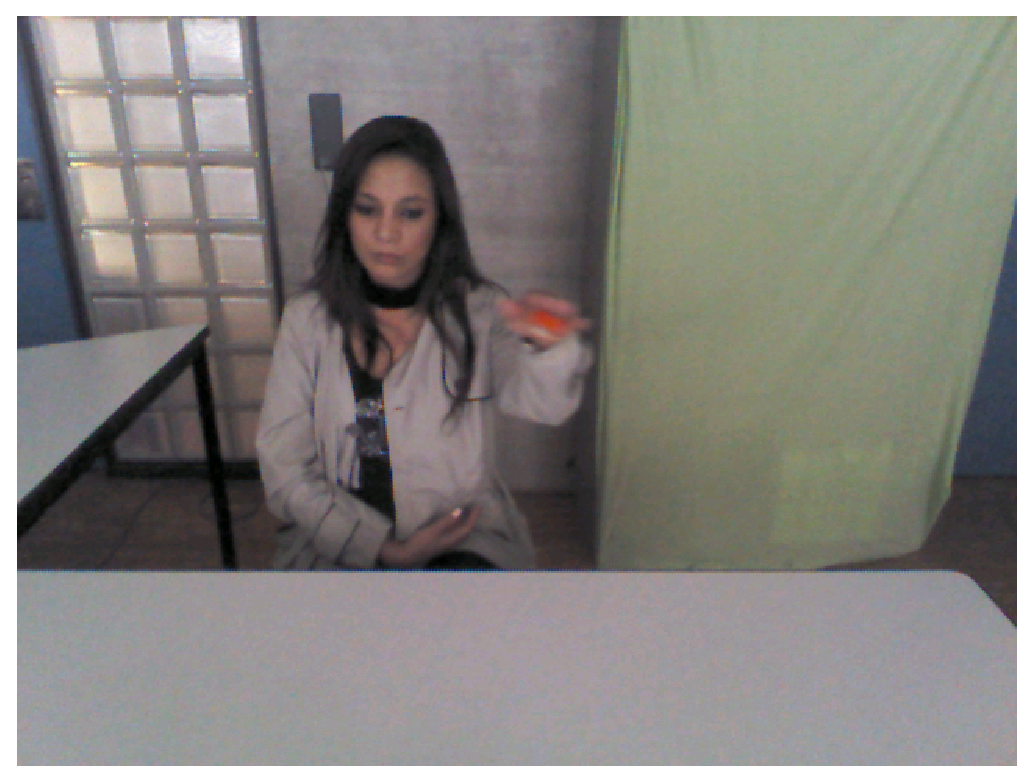
\includegraphics[width=0.19\linewidth]{fig/color.eps}\hspace{-0.6em}%
\label{fig:color}
}
\subfigure[]{
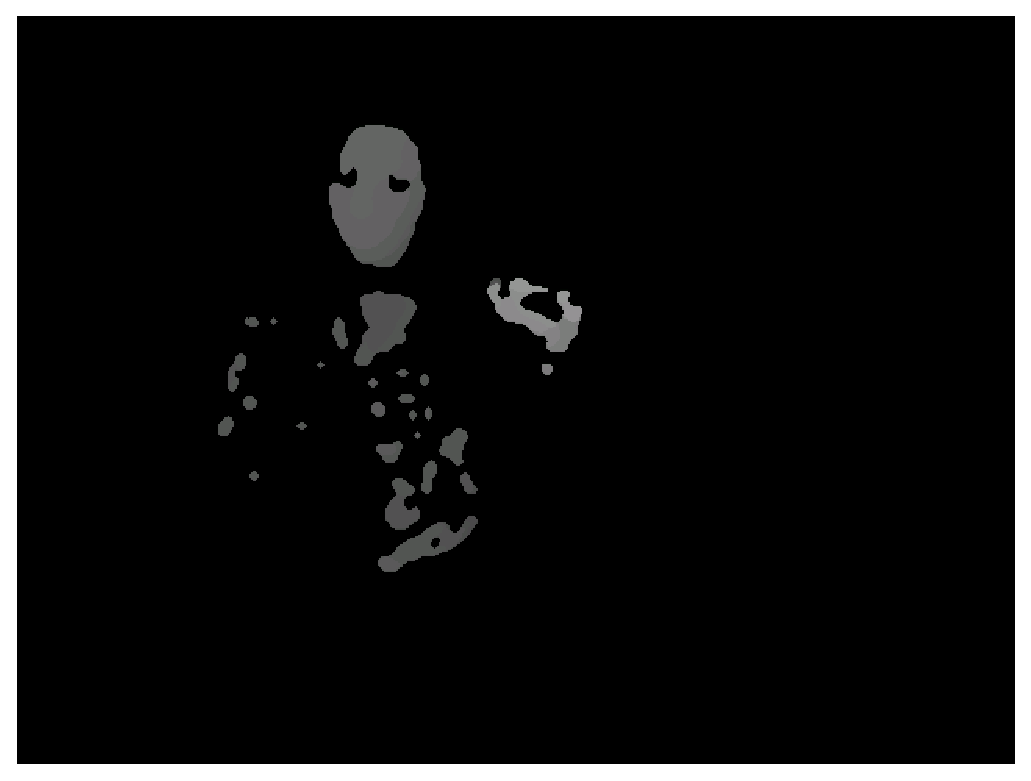
\includegraphics[width=0.19\linewidth]{fig/depth.eps}\hspace{-0.6em}
\label{fig:skin-mask}
}
\subfigure[]{
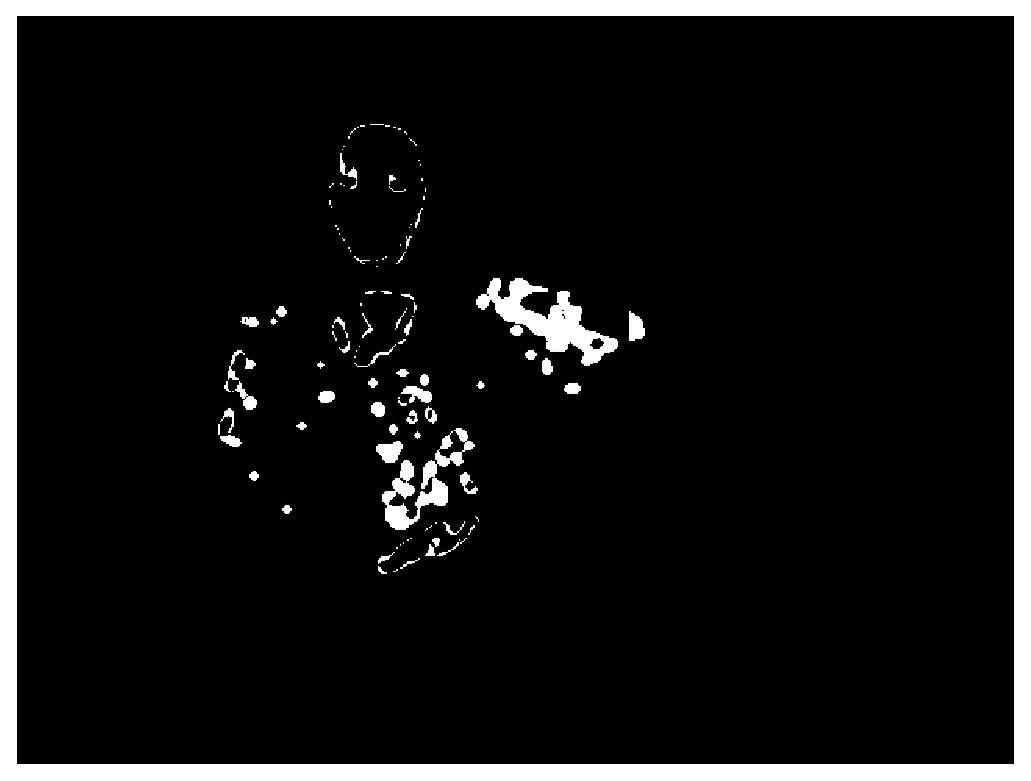
\includegraphics[width=0.19\linewidth]{fig/motion-mask1.eps}\hspace{-0.6em}
\label{fig:motion-mask}
}
\subfigure[]{
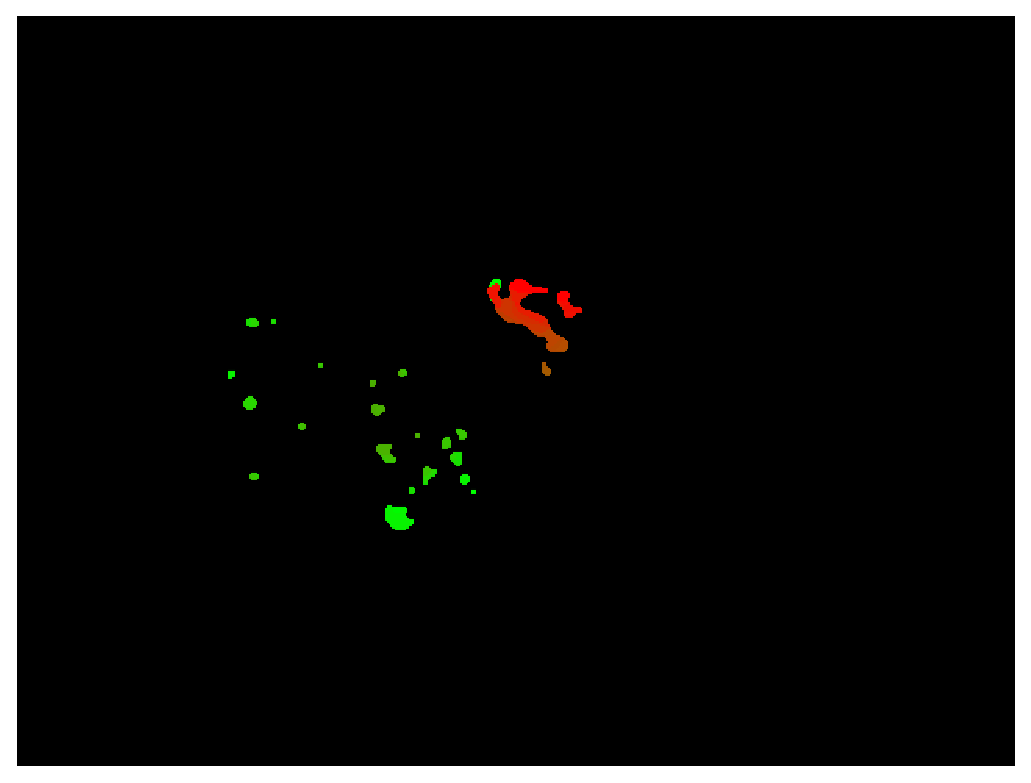
\includegraphics[width=0.19\linewidth]{fig/salient-map.eps}\hspace{-0.6em}
\label{fig:salience}
}
\subfigure[]{
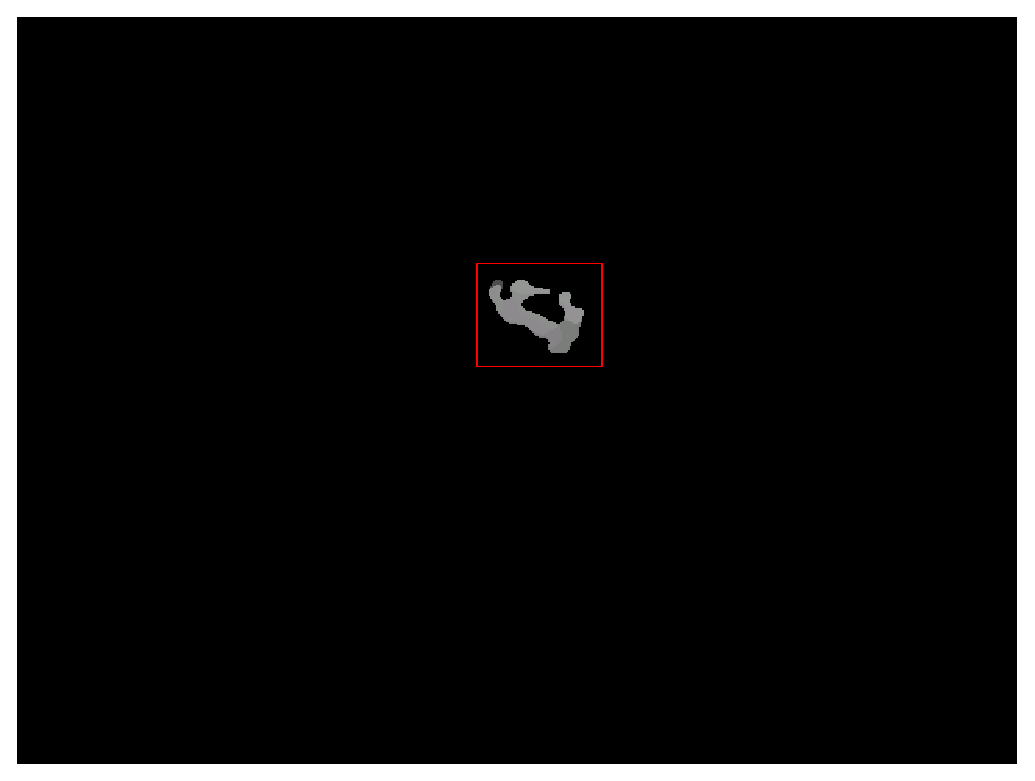
\includegraphics[width=0.19\linewidth]{fig/bounding-box.eps}
\label{fig:camshift}
}
\caption{Gesture salience detection steps: \subref{fig:color} RGB image under low lighting condition;
\subref{fig:skin-mask} depth map $D_t$ filtered by skin and user mask, $M_t^{S\wedge U}$. False detection of skin is due to
the similar colors between clothes and skin; \subref{fig:motion-mask} motion mask,  $M_{t\vee t-1}^M$, indicating moved pixels for time $t$ and $t-1$;
\subref{fig:salience} salience map with red color indicating high probability of the salience; 
\subref{fig:camshift} final gesture salience bounding box, $B_t$. (Best viewed in
color.)}
\label{fig:gesture-salience}
\end{figure*}

\subsubsection{Skin Segmentation}
We use an off-the-shelf simple skin color detection method to compute a binary skin mask at
time $t$, $M_t^S$, based on the RGB image. We also find the user mask, $M_t^U$ obtained from the Kinect SDK based on the depth image. 
We align the two to find their intersection $M_t^{S\wedge U}$, which indicates the user's skin region.

\subsubsection{Motion Detection}
We compute the motion mask for the current depth frame based on 3 frames. We first filter each 
depth frame by the user and skin mask $M_t^{S\wedge U}$, and then
smooth it through a median filter to obtain $D_t$ (Figure~\ref{fig:skin-mask}).
Equation~(\ref{eq:motion-mask}) computes the binary mask, $M_{t\vee t-1}^M$, 
indicating pixels whose depth values have changed from time $t-1$ to $t$ (Figure~\ref{fig:motion-mask}).
$D_{t\vee t-1}$ is the absolute difference between $D_t$ and $D_{t-1}$, and $T$ is the threshold operator that filters out small changes in depth value 
(with a threshold of 15mm). 
To obtain the motion mask, $M_{t}^M$ for time $t$ only, we use $M_{t-1\vee t-2}^M$, the motion mask for $t-1$ and $t-2$ as well (see Equation~(\ref{eq:motion-mask-t}),
 AND and XOR are indicated by $\wedge$ and $\oplus$).
\begin{align}
M_{t\vee t-1}^M &= T(D_{t\vee t-1}) \label{eq:motion-mask} \\
M_{t}^M &= M_{t\vee t-1}^M \oplus (M_{t\vee t-1}^M \wedge M_{t-1\vee t-2}^M) \label{eq:motion-mask-t}
\end{align}

\subsubsection{Salience Map}
We compute histograms of depth values in both $D_t$ and $D_{t\vee t-1}$ and then apply histogram normalization to obtain cumulative distributions $H_t$ and $H_{t\vee t-1}$.
$H_t$ represents the probability of salience given a depth value, while $H_{t\vee t-1}$ represents the probability of salience given
a depth difference value. The lower the depth value or the higher the depth difference value, the higher the salience probability. We use
histogram equalization to reduce the effect of outliers, so that a single large depth value will not suppress the salience probabilities of other depth values. 
The salience map (Figure~\ref{fig:salience}) can then be computed for each pixel $(x, y)$:
\begin{align*}
S_t(x, y) = H_t(D_t(x, y)) \times H_{t\vee t-1}(D_{t\vee t-1}(x, y)) \times M_t^M
\end{align*}
The multiplication of the binary motion mask $M_t^M$ allows us to consider only the motion due to the user at $t$.
 
\subsubsection{Salience Location}
The final step of locating the most salient region in a frame is finding the
contour, $C_t$, from the salience map $S_t$ that has a perimeter greater than
the smallest possible hand perimeter and with the highest average salience for all the pixels inside the contour.

When motion is slow, the motion mask usually indicates the edge of the moving
object. As a result, the center of $C_t$ may not be the center of the moving
object (in our case, the user's hand). Hence, we use 2 iterations of Camshift~\cite{Bradski98} on 
the depth image $D_t$ with a starting search location at the center of $C_t$ to refine
the final bounding box, $B_t$, of gesture salience (Figure~\ref{fig:camshift}). Figure~\ref{fig:compare-skeleton} compares the hand detection result using our method with that using the skeleton tracking result
from the Kinect SDK.
\begin{figure*}
\centering
\subfigure[]{
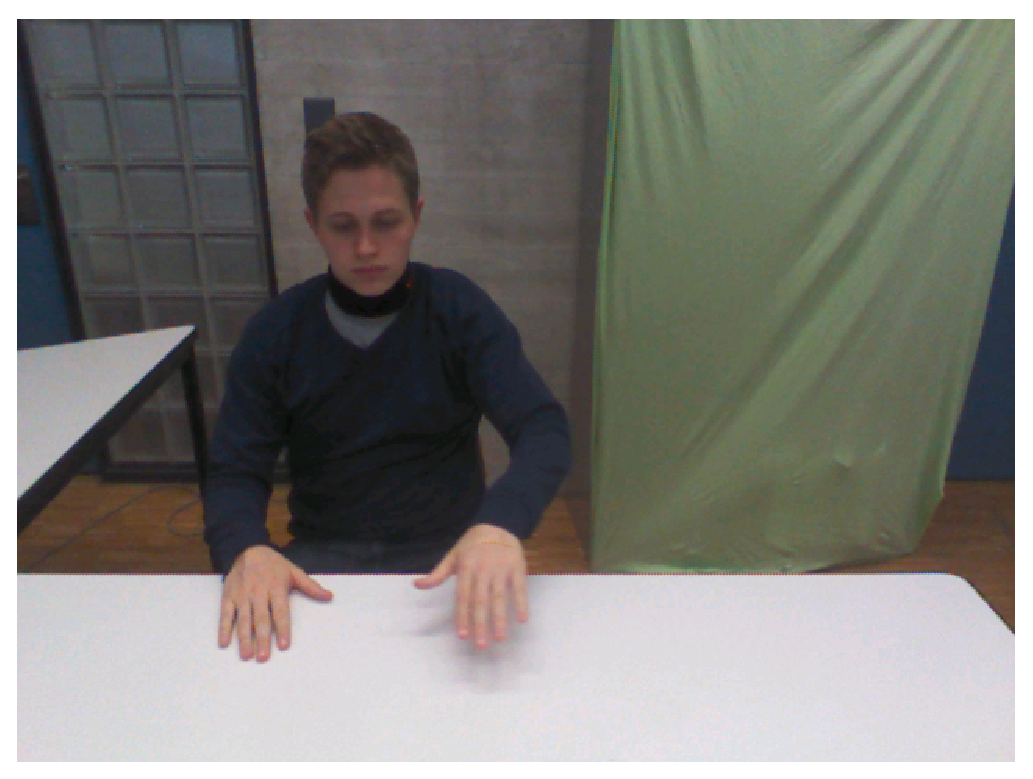
\includegraphics[width=0.23\linewidth]{fig/rotate-color.eps} \hspace{-0.6em}
}
\subfigure[]{
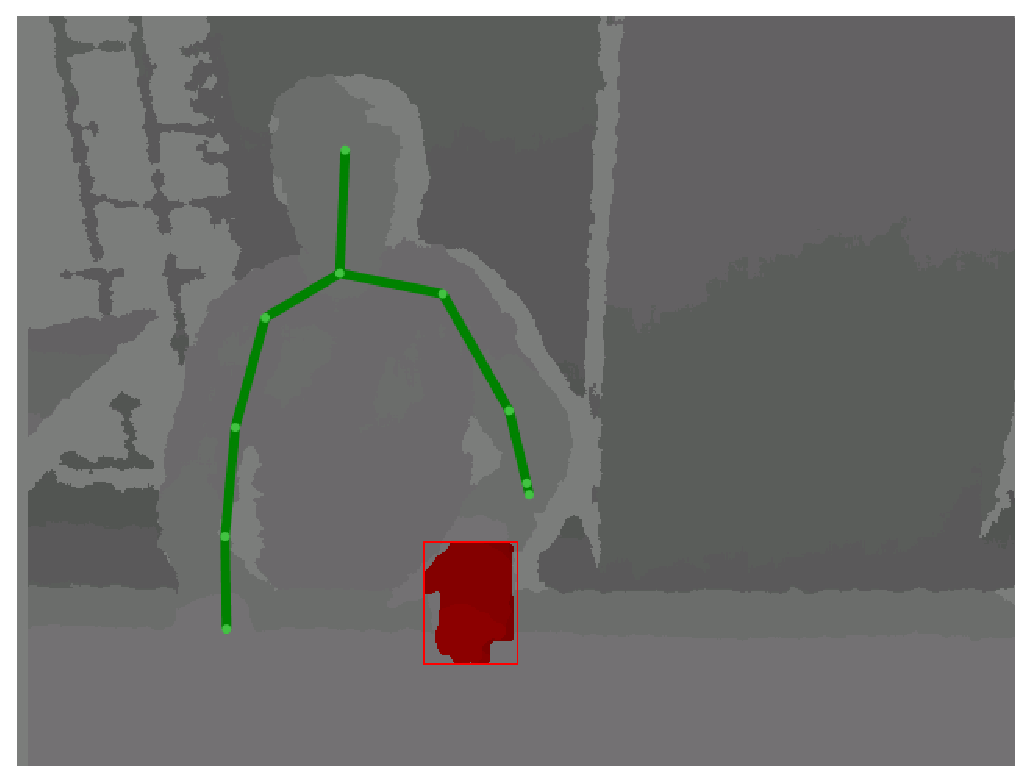
\includegraphics[width=0.23\linewidth]{fig/rotate-depth.eps} \hspace{-0.6em}
}
\subfigure[]{
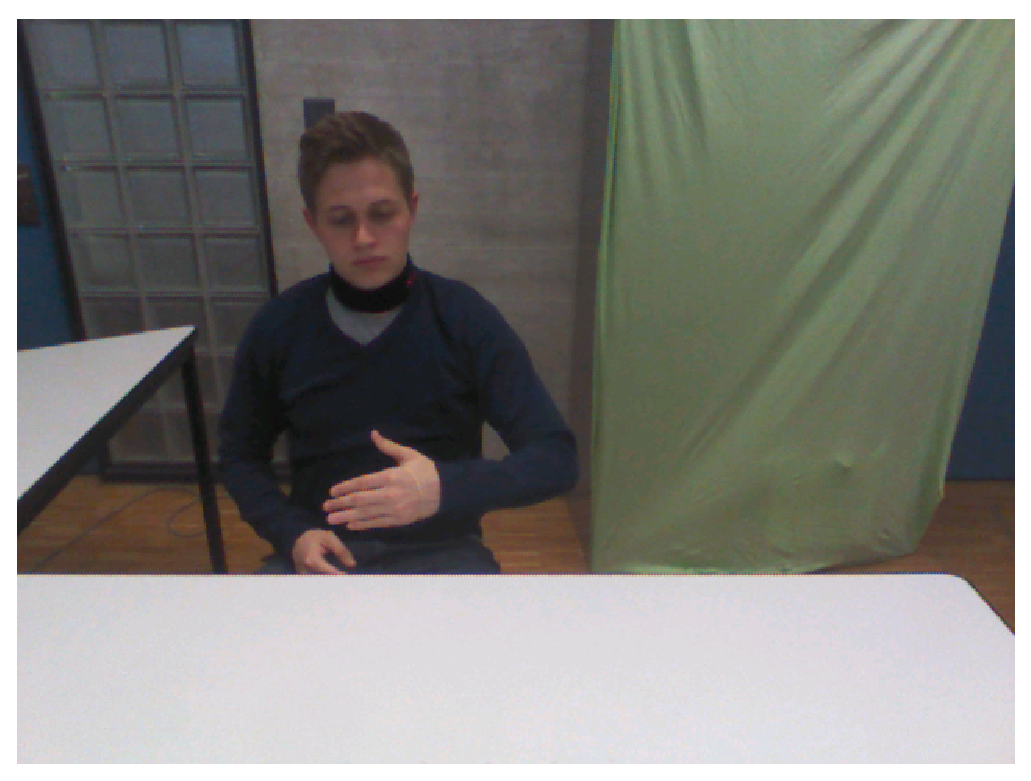
\includegraphics[width=0.23\linewidth]{fig/near-body-color.eps}
\hspace{-0.6em} }
\subfigure[]{
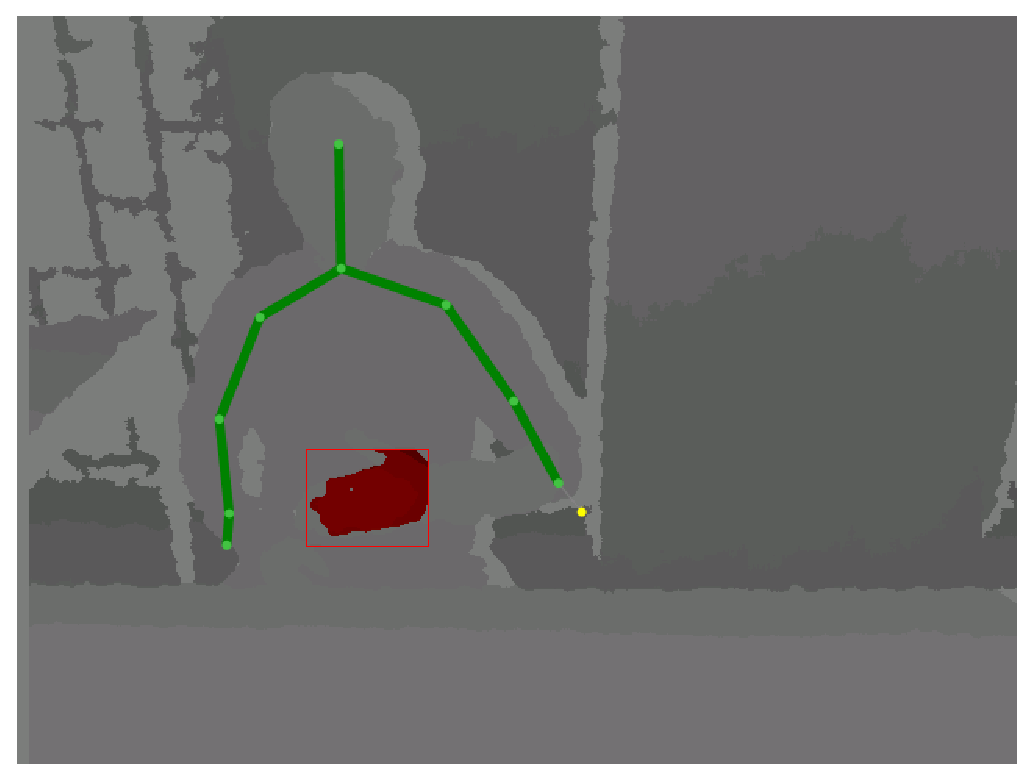
\includegraphics[width=0.23\linewidth]{fig/near-body-depth.eps}
\hspace{-0.6em} }
\caption{Comparison of hand detection using our gesture salience method versus using the skeleton tracking from the Kinect SDK. The green lines are
the skeleton tracking results. The red region is the salient gesture
region using our method. (Best viewed in color.)}
\label{fig:compare-skeleton}
\end{figure*}

\section{Temporal Segmentation}\label{sec:recognition}
We used all the training data from all the users to create a Gaussian model for the rest 
positions and a Gaussian model for non-rest positions.

During recognition, an observation $\underline{x}_t$ is first classified as a 
rest or a non-rest position. It is a non-rest position if 
\begin{displaymath}
N(\underline{x}_t; \mu_{\text{NON-REST}}, \Sigma_{\text{NON-REST}}) \geq N(\underline{x}_t; \mu_{\text{REST}}, \Sigma_{\text{REST}})
\end{displaymath}
where $N$ represents the Gaussian probability. Sequences of continuous observations from non-rest
positions longer than 0.25s are further classified into different gestures based on trained HMMs.
 
\section{Gesture Spotting and Recognition}
\subsection{Temporal Gesture Modeling and Training}
Previous research suggests that
a gesture consists of three phases: \textit{pre-stroke}, \textit{nucleus}, and \textit{post-stroke}~\cite{Pavlovic97}. The pre-stroke phase consists
of a preparatory movement that sets the hand in motion from some resting position.
The nucleus of a gesture has some ``definite form and enhanced dynamic qualities''
~\cite{kendon86}. Finally, the hand either returns to the resting position or repositions
for the new gesture phase. Each gesture
phase includes a sequence of hand/arm movement that can be modeled using HMMs (see Figure~\ref{fig:hmm}). 

\begin{figure}[tb]
\centering
\includegraphics[clip, width=1\columnwidth]{fig/hmm.ps}
\caption{Temporal gesture model with different phases. Each phase can be modeled as an HMM. Dashed arrows represent
initial state transitions and double circles
represent end states.}
\label{fig:hmm}
\end{figure}

Because we have the ground truth labeling of pre-stroke, nucleus and post-stroke phases, 
we can train an HMM for each phase for each gesture. 

As each phase can have variable length, we model the termination probability for each
hidden state $s$ as $t(\text{END}|s)$. Given a sequence of observation $\underline{X}_1^T = \underline{x}_1\ldots\underline{x}_T$, and 
the corresponding hidden states sequence $S_1^T = s_1\ldots s_T$, we define the probability
\begin{displaymath}
p(\underline{X}_1^T, S_1^T;\underline{\theta}) = 
    t(s_1)t(END|s_T)\prod_{t = 2}^T t(s_t | s_{t-1})\prod_{t = 1}^T e(\underline{x}_t|s_t)
\end{displaymath}
where $\underline{\theta}$ represents the model parameter vector which includes
the initial state probabilities $t(s)$, the state transition probabilities $t(s'|s)$, and the 
emission probabilities $e(\underline{x}|s)$ for $s, s'\in \{1, 2,\ldots k\}$. We use a mixture of 3 Gaussians for the emission probability to model user variations.

Given $N$ training sequences, we use the expectation maximization (EM) algorithm to estimate the model parameters. In
particular, the update for the termination probability during the $i$th iteration is 
\begin{displaymath}
t^i(END|s) = \frac{\sum_{j = 1}^N \overline{count}(j, s\rightarrow END;\underline{\theta}^{i-1})}
    {\sum_{j = 1}^N\sum_{s'} \overline{count}(j, s\rightarrow s';\underline{\theta}^{i-1})}
\end{displaymath}
where $\overline{count}(j, s\rightarrow END;\underline{\theta}^{i-1})$ is the expected count of 
$s$ being the end state. We can use the usual forward-backward algorithm to compute all the 
expected sufficient statistics by adding a dummy END state to the end of each sequence.

Because there are 3 rest positions, we use 3 hidden states for both the pre-stroke and post-stroke phases.
Each hidden state can be the start state and can only remain in its own state or go to the end state.
 
For the nucleus phase, we use 6 hidden states for all the gestures and use a modified Bakis~\cite{bauer2000} model to constrain the transition probabilities
among the hidden states. Instead of allowing only left-right transition, we allow the last hidden state
to go back to the initial state (Figure~\ref{fig:bakis}). This is particularly important for modeling gestures with arbitrary number of
repetitions such as waving and shaking hands. 

\tikzstyle{vertex}=[circle, draw, minimum size=16pt, inner sep=0pt]
\tikzstyle{observed-vertex}=[circle, draw, minimum size=16pt, inner
sep=0pt, fill=black!20] 
\tikzstyle{edge} = [draw, thick, -]
\tikzstyle{directed-edge} = [draw, ->]

\begin{figure}[tb]
\centering
  \begin{tikzpicture}[auto,swap, scale=1.5]
    % First we draw the vertices
    \foreach \pos/\name in {{(0, 0)/start}, {(1, 0)/s_1}, {(2, 0)/s_2},
    {(3, 0)/s_3}, {(4, 0)/s_4}, {(5, 0)/end}}
      \node[vertex] (\name) at \pos {$\name$};
    % Connect vertices with edges and draw weights
    \foreach \source/ \dest in {s_2/s_3, s_3/s_4, s_4/end,
    s_1/s_2} \path[directed-edge] (\source) -- (\dest);
    
    \foreach \source/ \dest in {s_1/s_3, start/s_2, s_2/s_4, s_3/end, s_4/s_1} 
      \path[directed-edge] (\source) edge [bend left] (\dest);
      
    \foreach \source/ \dest in {s_1/s_1, s_2/s_2, s_3/s_3, s_4/s_4} 
      \path[directed-edge] (\source) edge [loop above] (\dest);
    
    \path[directed-edge] (start) edge node [below] {$t(s_1)$} (s_1);
  \end{tikzpicture}
  \caption{A state transition diagram of a modified 4-state Bakis model for the nucleus phase.}
  \label{fig:bakis}
\end{figure}

\subsection{Gesture Recognition}
During the recognition phase, we concatenate the HMMs trained for each phase together to form
one HMM for each gesture. The transition probability from the previous phase to the next
phase can be computed by multiplying the termination probabilities of the previous phase and the
initial state probabilities of the next phase. Using the superscript $c$ to denote the model
parameters in the concatenated HMM, we have
\begin{displaymath}
t^c(s_\text{nucleus}|s_\text{prestroke}) = t(\text{END}|s_\text{prestroke}) \times t(s_\text{nucleus})
\end{displaymath}
where $s_{\text{phase}}$ denotes the hidden state variable in a particular phase. We add small transition
probabilities from the pre-stroke phase to the post-stroke phase to model movements that do not have the 
nucleus phase.

As new state transition probabilities are added, the transition probabilities among
states in the same phase also need to be modified so that $\sum_{s' = 1}^K t(s'|s) = 1$ (where
$K$ is the total number of combined hidden states) is ensured. For example
\begin{displaymath}
t^c(s'_{\text{nucleus}} | s_{\text{nucleus}}) = t(s'_{\text{nucleus}} | s_{\text{nucleus}})
  \times (1 - t(\text{END} | s_{\text{nucleus}}))
\end{displaymath}

We also add a rest state to the end of the HMM and allow the rest state to transit to the pre-stroke
and the post-stroke phase with uniform probabilities (Figure~\ref{fig:hmm}) to accommodate short pauses during the gesture.
As a result, the final HMM for each gesture has 13 hidden states.
Let $\underline{\theta}_g$ be the final concatenated HMM parameters for gesture $g$. The classification
of an observation sequence from non-rest positions is 
\begin{displaymath}
\hat{g} = \arg\max_g\log p(\underline{X}_1^T; \underline{\theta}_g)
\end{displaymath}

\subsection{Gesture Spotting}
Because the non-rest positions include both pre-stroke and post-stroke phases, we need
to detect the start of the actual gesture (nucleus). We use the Viterbi algorithm
to find the most probable hidden state sequence $\hat{s}_1\ldots\hat{s}_T$ for a given observed sequence using 
the mostly likely gesture model $\underline{\theta}_{\hat{g}}$. The start and the end time for a gesture nucleus are
the first and the last time frame $t$ where $\hat{s}_t\in s_{\text{nucleus}}$ respectively. Note that
we are able to identify whether a hidden state belongs to the nucleus phase because we trained the three phases
separately.

\begin{figure}[tb]
\centering
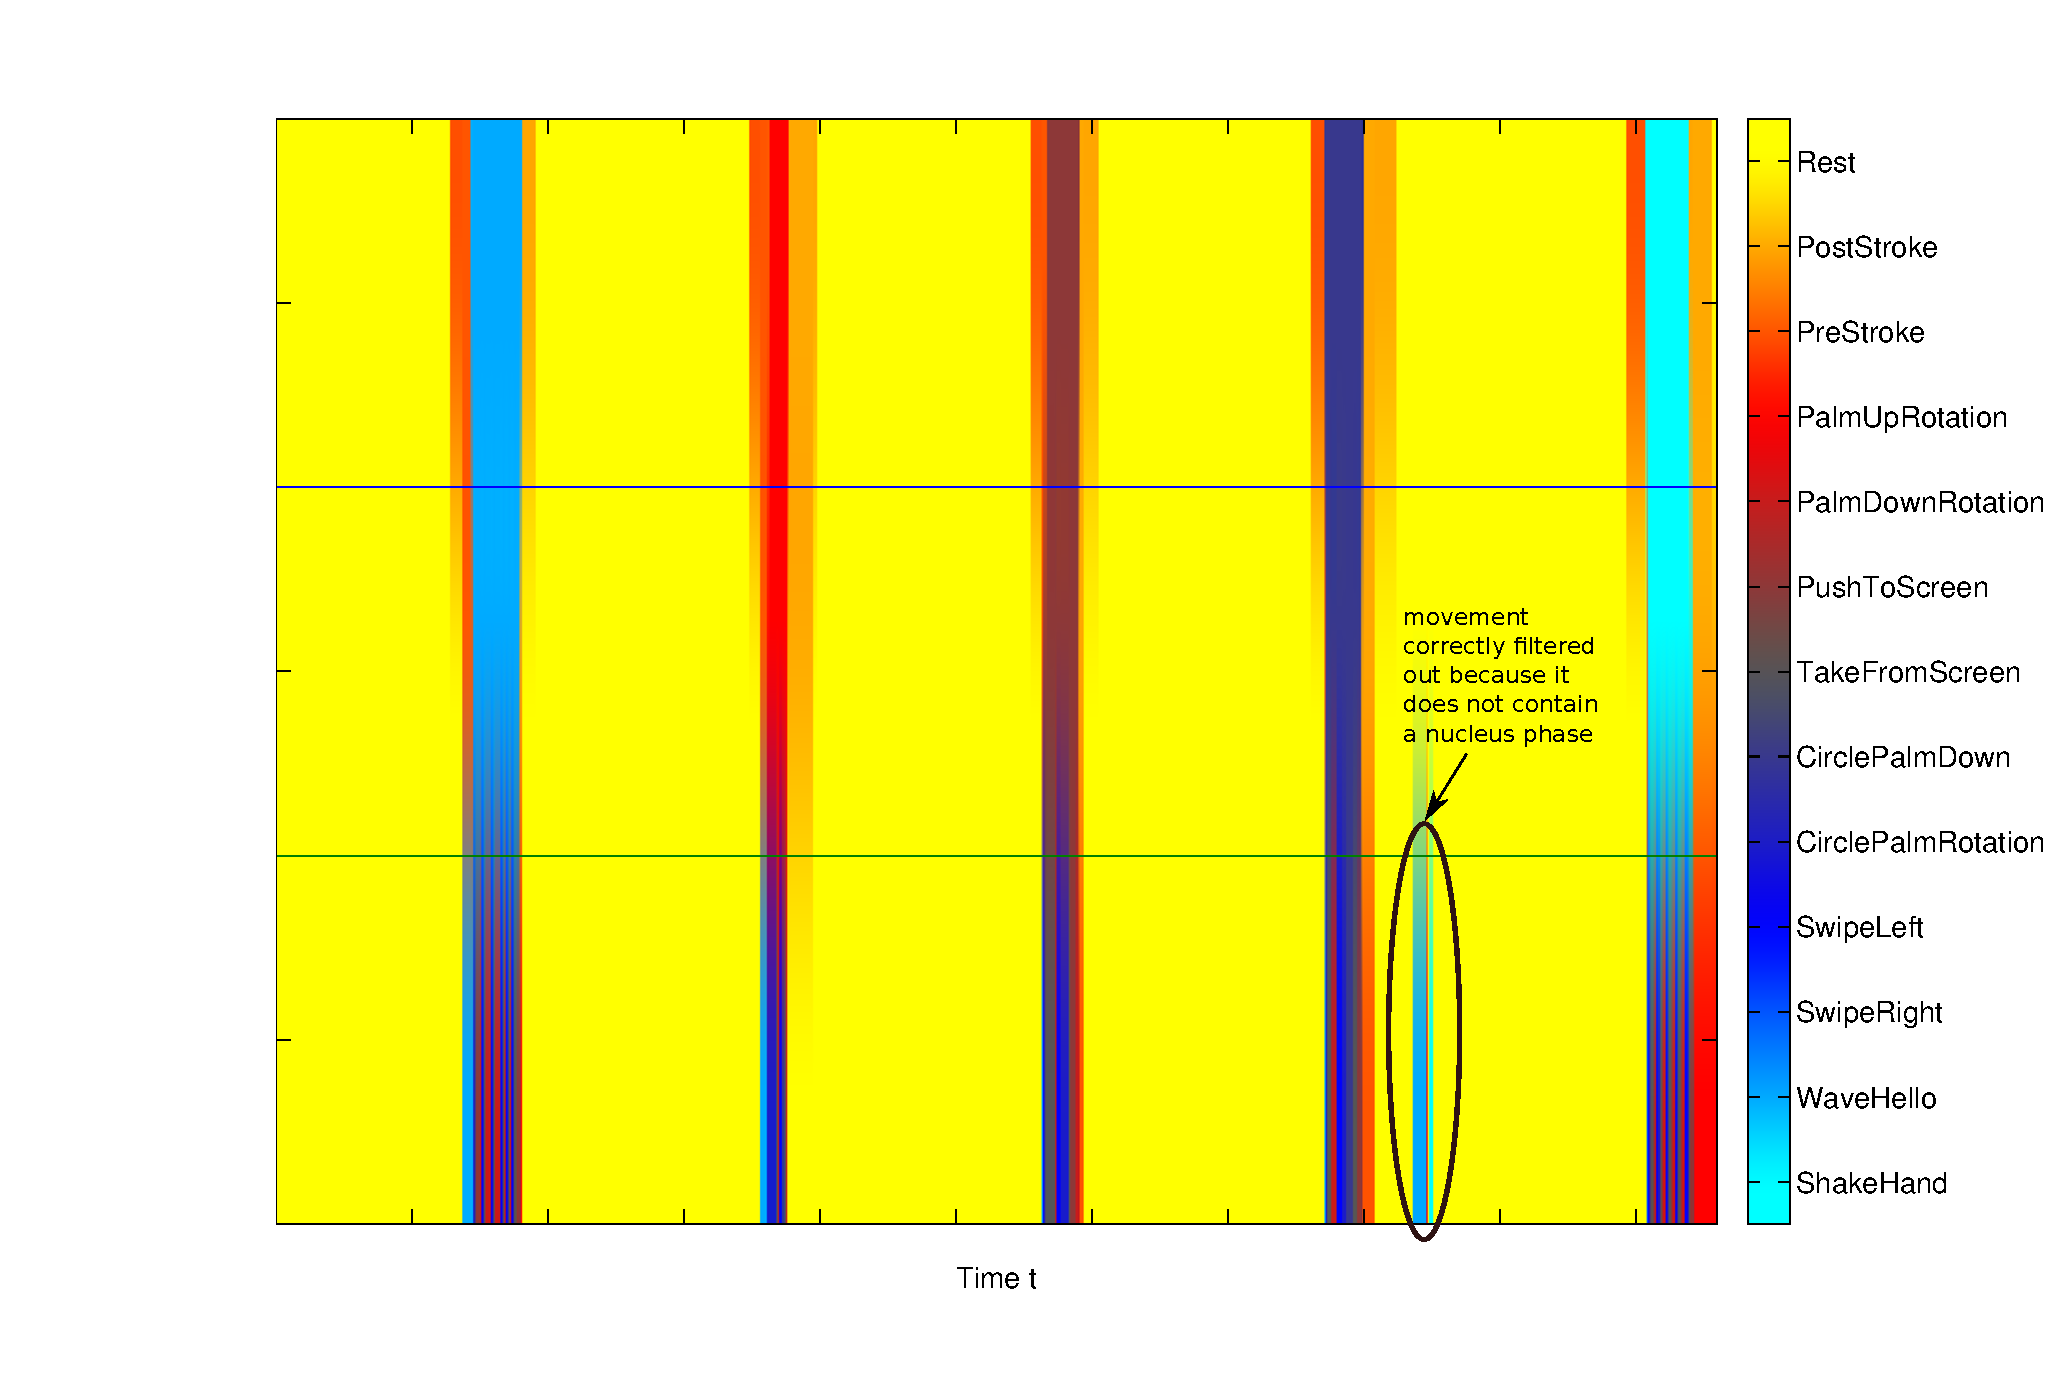
\includegraphics[trim={3.5cm 1.4cm 0cm 0.6cm}, clip, width=1\columnwidth]{fig/01-3-3.ps}
\caption{Visualization of a gesture recognition sequence. 
The pre-stroke and post-stroke phases are indicated by two orange colors (see the color bar). 
The colors for the hidden states (3rd row) are not related 
to the gestures. Instead the first 3 blues in the color bar are for the pre-stroke hidden states, the next 6 colors are for the nucleus, 
the next 3 are for the post-stroke, and the last is for the rest state.}
\label{fig:decoding}
\end{figure}

Figure~\ref{fig:decoding} shows a recognition result visualization for one batch sequence. The first
row is the ground truth with different colors indicating different gesture phases or the rest position. 
The second row is our segmentation and recognition result.
The third row is the color-coded most probable hidden states. If a non-rest sequence does not contain hidden states belonging to the nucleus phase, 
it is ignored (see the blue bar at $t\sim 30700$ in Figure~\ref{fig:decoding}). In
this way, we can spot the actual gestures while filtering out other movements.
\pagebreak
\section{Experimental Evaluation}\label{sec:eval}
We evaluate our method based on the development data set, and down sample the frame rate
to 12.5Hz.
Table~\ref{tab:comp-feature} shows the average result of a 3-fold cross validation where, in each fold,
the model is trained on 2 sessions and tested on 1 session from every user. We compare
the result based on two different feature vectors: using both Kinect and Xsens features versus using
only Xsens features. The result shows that including the relative hand position computed from 
the Kinect data improves the F1 score by 1.3\%. 

The confusion matrix (Figure~\ref{fig:confusion}) shows that the most easily confused gestures
are ``take from screen'' and ``push to screen''. These two gestures are very similar except for hand
poses. This suggest that by including hand pose features may further improve
the recognition accuracy.

\begin{table}[tb]
\begin{center}
\begin{tabular}{|l|l|l|}
\hline
 & Kinect \& Xsens & Xsens Only \\
\hline
F1 Score & \textbf{0.900} & 0.887 \\
\hline
ATSR Score & \textbf{0.923} & 0.917 \\
\hline
Final Score & \textbf{0.9012} & 0.8932 \\
\hline
\end{tabular}
\caption{Comparison of the average 3-fold cross validation results for two feature vectors:
using both Kinect and Xsens features versus using only Xsens featurs. }
\label{tab:comp-feature}
\end{center}
\end{table}

\begin{figure}[tb]
\centering
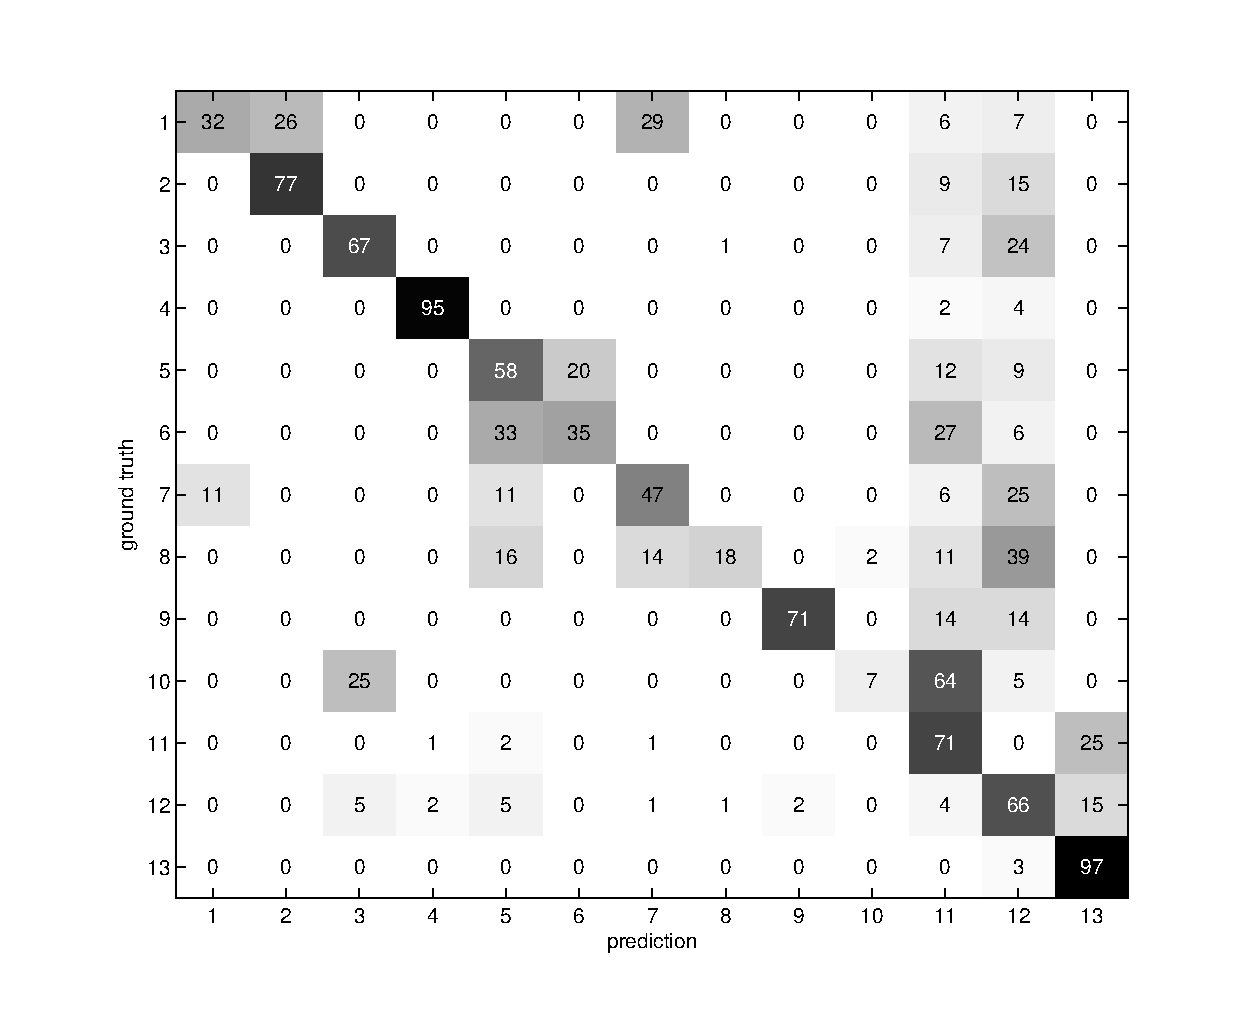
\includegraphics[trim={6cm 3.5cm 10cm 1.5cm}, clip, width=1\columnwidth]{fig/confusion-matrix.eps}
\caption{Confusion matrix based on result from 3-fold cross validation using both Kinect and Xsens
features. The numbers are percentages. The darker the color the higher the percentage.}
\label{fig:confusion}
\end{figure}

\begin{table}[tb]
\begin{center}
\begin{tabular}{|l|l|l|l|l|l|}
\hline
Hit & 843 & Missed & 49 & Mislabel & 7 \\
\hline
Precision & 0.94 & Recall & 0.94 & F1 & 0.90\\
\hline
Start error & 0.3\% & Stop error & -2.33\% & ATSR & 0.92  \\
\hline
\multicolumn{5}{|r|} {\textbf{Final Score}} & \textbf{0.9357}  \\
\hline
\end{tabular}
\caption{Training result using all the development data.}
\label{tab:dev-score}
\end{center}
\end{table}

Using both the Kinect and the Xsens features, we also trained a model using all the development data (Table~\ref{tab:dev-score}). 

\section{Conclusions}
Our gesture spotting method based on concatenated HMMs trained for the three gesture phases
and Viterbi decoding gives a good result on the development data set. Using hand position features computed from
Kinect data also helps to increase the gesture recognition accuracy. 
 
%\end{document}  % This is where a 'short' article might terminate

% The following two commands are all you need in the
% initial runs of your .tex file to
% produce the bibliography for the citations in your paper.
\bibliographystyle{abbrv}
\bibliography{sigproc}  % sigproc.bib is the name of the Bibliography in this case
% You must have a proper ".bib" file
%  and remember to run:
% latex bibtex latex latex
% to resolve all references
%

\balancecolumns % GM June 2007
% That's all folks!
\end{document}
